\documentclass[10pt,a4paper]{article}
\usepackage[utf8]{inputenc}
\usepackage[T1]{fontenc}
\usepackage{lmodern}
\usepackage[margin=1.5cm, top=1.4cm, bottom=1.4cm]{geometry}
\usepackage{hyperref}
\usepackage{enumitem}
\usepackage{titlesec}
\usepackage{xcolor}
\usepackage{graphicx}

\definecolor{accent}{HTML}{00686E}
\hypersetup{colorlinks=true, urlcolor=accent, linkcolor=accent}
\pagenumbering{arabic}
\setlength{\parindent}{0pt}

\titleformat{\section}{\large\bfseries\color{accent}}{}{0em}{}[\vspace{-0.6em}\rule{\textwidth}{0.8pt}]
\titlespacing{\section}{0pt}{7pt}{4pt}

\newcommand{\role}[4]{%
  \textbf{#1} \hfill \textbf{#2}\\[1pt]%
  \textit{#3} \hfill \textit{#4}\\[2pt]%
}
\setlist[itemize]{leftmargin=1.2em, itemsep=1.5pt, topsep=2pt, parsep=0pt}

\begin{document}

% ================= HEADER =================
\begin{minipage}[c]{0.80\textwidth}
  {\Huge\bfseries Prabhavit Gupta}\\[3pt]
  {\color{accent}\large AI Engineer: RAG Architectures, Agent Workflows \& Enterprise AI Platforms}\\[6pt]
  {\footnotesize +39 351 610 7807 ~$\vert$~
  \href{mailto:prabhavitg@gmail.com}{prabhavitg@gmail.com} ~$\vert$~
  \href{https://www.linkedin.com/in/prabhavit/}{linkedin.com/in/prabhavit} ~$\vert$~
  \href{https://github.com/prab-gupta}{github.com/prab-gupta} ~$\vert$~
  Venice, Italy (EU Permanent Resident / Global Remote Ready)}
\end{minipage}\hfill
\begin{minipage}[c]{0.18\textwidth}
  \raggedleft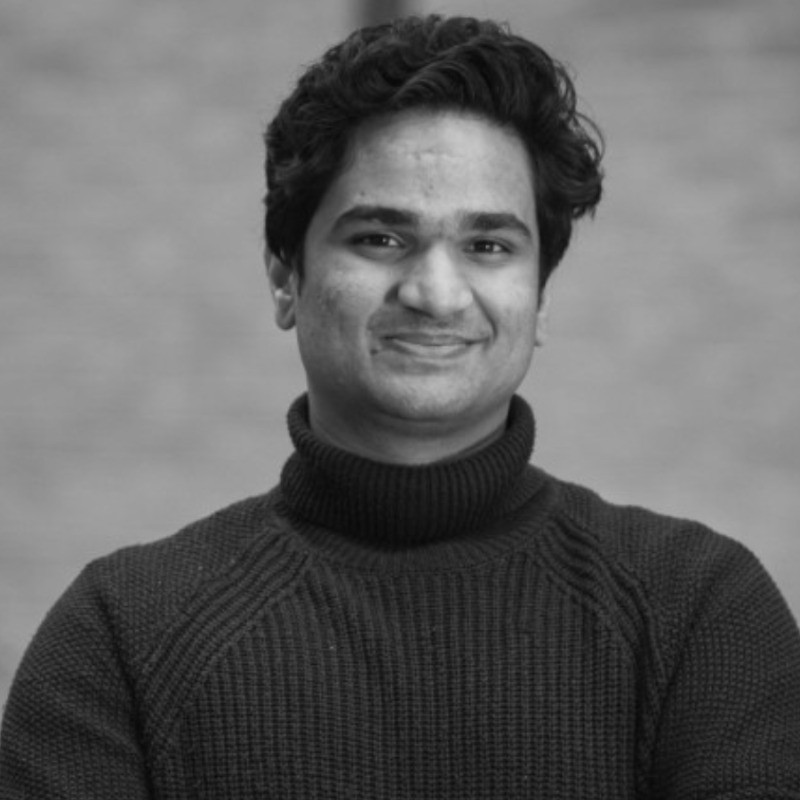
\includegraphics[width=2.0cm]{photo.jpg}
\end{minipage}
\vspace{-2pt}

% ================= SUMMARY =================
\section{Summary}
AI Engineer with 3 years of hands-on software and systems engineering experience architecting, shipping, and operating production RAG pipelines, enterprise agent workflows, and tool-augmented LLM applications. Deep practical expertise in end-to-end retrieval architectures (semantic chunking, hybrid search, metadata filtering, pgvector indexing, reranking), tool integrations via Model Context Protocol (MCP) and REST APIs, and automated evaluation harnesses measuring grounding, precision, and latency. Proven ability to translate enterprise knowledge and data security constraints into reliable, traceable AI workflows with human-in-the-loop approvals. Holder of an EU Long-Term Residence Permit (permanent unrestricted EU work authorization across all EU member states, no sponsorship required); based in Venice, Italy and available immediately for worldwide remote freelance contracts.

% ================= TECHNICAL EXPERTISE =================
\section{Technical Expertise}
\begin{itemize}
  \item \textbf{RAG Architectures \& Vector Retrieval:} Chunking strategies, hybrid search (dense + BM25 sparse), vector embeddings, PostgreSQL with \texttt{pgvector}, metadata filtering, cross-encoder reranking, context window management, citation grounding.
  \item \textbf{Agent Workflows \& LLM Integration:} Tool-calling architectures, Model Context Protocol (MCP), multi-turn agent execution, human-in-the-loop approval gates, structured JSON extraction, OpenAI, Anthropic, and open-weights LLMs.
  \item \textbf{Evaluation \& Observability:} Ground-truth benchmark datasets, retrieval quality metrics (precision@k, recall@k), LLM-as-a-judge grounding verification, latency and token cost optimization, transcript audit logging.
  \item \textbf{Software Development \& Backend Systems:} Python (FastAPI, asyncio), TypeScript, Node.js, RESTful APIs, webhook orchestration, PostgreSQL schema modeling, Redis asynchronous task queues.
  \item \textbf{Cloud, DevOps \& Quality Assurance:} Docker containerization, CI/CD pipelines, Git version control, automated regression and contract testing with Playwright, Linux server management.
  \item \textbf{Languages \& Authorization:} English (C1 Professional, fluent), Hindi (Native), Italian (Beginner). EU Long-Term Residence Permit (unrestricted EU work authorization across all EU member states, no visa sponsorship required).
\end{itemize}

% ================= EXPERIENCE =================
\section{Experience}

\role{\href{https://flowspace.co}{FlowSpace.co}}{Mar 2024 - Aug 2026}{Lead Developer \& AI Systems Architect}{London, UK (remote)}
\begin{itemize}
  \item Designed and operated production customer-facing AI agents and retrieval systems for a platform serving 4,500+ active enterprise users, enabling natural language search and action execution across catalog APIs.
  \item Implemented robust document ingestion and extraction pipelines using LLMs and structured parsing, converting messy unstructured partner inventories into validated JSON schemas.
  \item Built multi-step agent reasoning chains with strict tool execution constraints, schema validation, and human-in-the-loop approval checkpoints, ensuring zero ungrounded actions in customer-facing flows.
  \item Engineered automated evaluation harnesses evaluating retrieval precision and response accuracy against real user conversation transcripts, reducing edge-case hallucination and fallback rates.
  \item Architected and maintained resilient TypeScript/Node.js backend services and PostgreSQL data layers, utilizing asynchronous Redis queues to handle high-throughput query spikes.
  \item Developed automated integration and end-to-end regression test suites with Playwright, enforcing strict API contract adherence and zero functional regressions across continuous deployment cycles.
\end{itemize}

\role{Urlink}{Apr 2025 - Jul 2025}{Project Manager \& Solutions Developer (Freelance)}{Barcelona, Spain (remote)}
\begin{itemize}
  \item Led technical discovery and implementation of customized web applications, data processing pipelines, and external API connectors for client platforms.
  \item Built automated data ingestion and transformation services connecting third-party partner APIs to PostgreSQL databases, maintaining strict data integrity and schema validation.
  \item Shipped interactive prototypes and API test harnesses to validate system boundaries and data flows prior to sprint execution, accelerating delivery timelines.
\end{itemize}

\role{Independent Technical Consultant}{Aug 2023 - Feb 2024}{AI Automation \& Integration Developer}{Venice, Italy}
\begin{itemize}
  \item Built and deployed custom LLM integrations, document retrieval prototypes, and webhook automation workflows for European enterprise clients using Python, TypeScript, and n8n.
  \item Replaced brittle manual document review workflows with automated LLM-assisted classification and extraction pipelines featuring comprehensive error handling and fallback routing.
  \item Authored technical architecture specifications, API documentation, and deployment guides to support client engineering teams in operating self-hosted workflows.
\end{itemize}

% ================= EDUCATION =================
\section{Education}
\role{Ca' Foscari University of Venice}{2020 - 2024}{BA in Philosophy, International Studies and Economics}{Venice, Italy}
\begin{itemize}
  \item Rigorous training in formal logic, epistemology, analytical problem solving, systems analysis, and macroeconomic decision models.
\end{itemize}

\end{document}
